
\begin{exercise}
% !TEX root = ../main.tex


\pt{4}In de figuur zie je zes bewegingen van een bal die van links naar rechts beweegt. De pijlen geven de positieve richting oftewel de $x$-as aan. Elke cirkel stelt de positie van de bal voor op opeenvolgende tijdstippen. De tijdsintervallen tussen die opeenvolgende tijdstippen zijn gelijk.
\begin{figure}[hbt]
	\begin{flushright}
	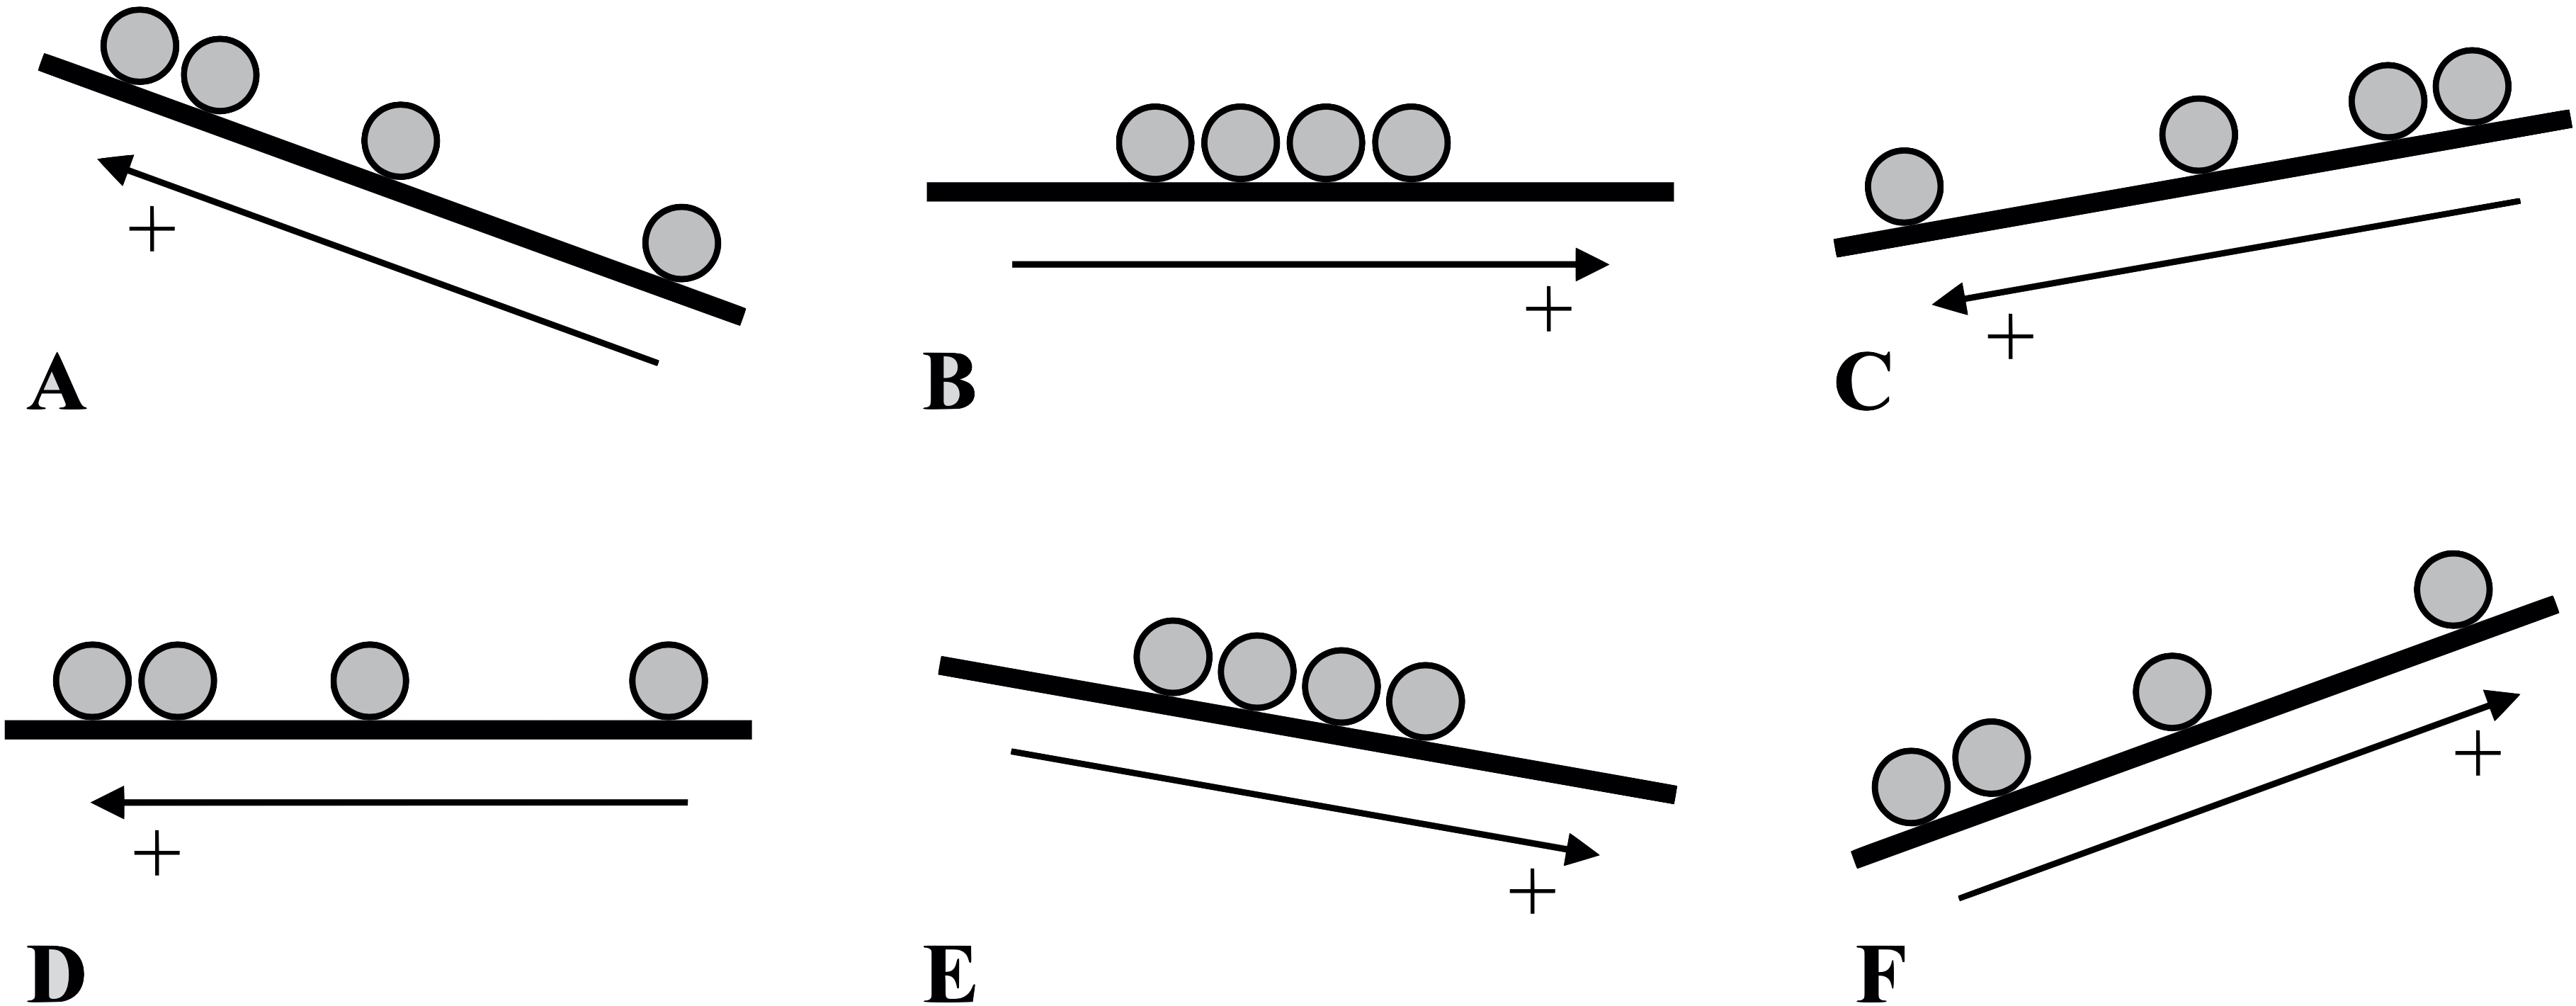
\includegraphics[width=.93\textwidth]{hb_natuurkundedidactiek_34}
	%\includegraphics[height=\textheight]{}
	%\caption{}
	\end{flushright}
\end{figure}
\begin{enumerate}
\item Zet de bewegingen op volgorde op basis van de eindsnelheid van de bal. Begin met de beweging waarbij die eindsnelheid het grootst is. Let op: nul is groter dan negatief.
\item Doe hetzelfde als in (a) maar nu voor de versnelling van de bal.% (in plaats van de eindsnelheid). %Zet de bewegingen op volgorde op basis van de versnelling van de bal. Begin met de beweging waarbij die versnelling het grootst is. Let op: nul is groter dan negatief.
\end{enumerate}
Als er twee of meer situaties zijn die gelijk ‘scoren’, dan komen die situaties op dezelfde plaats in jouw volgorde te staan. Je geeft dat aan door ze bijvoorbeeld te omcirkelen. %Leg ten slotte de redenering achter jouw volgorde uit.

\begin{oplossing}
	(a) F, B=E, C, A=D
	
	(b) F=C, B=E, A=D
\end{oplossing}

\end{exercise}
